\begin{figure}
    \centering
    \begin{tabular}{ll}
        \textbf{(a)} & \textbf{(b)} \\
        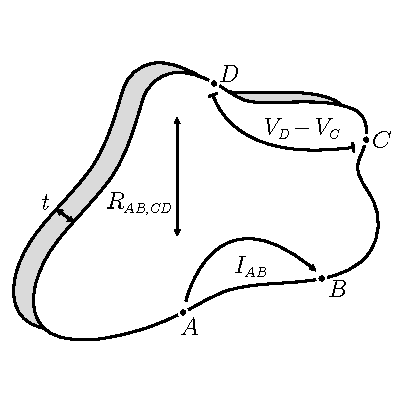
\includegraphics[align=c]{vanDerPauw.pdf}
        & \includegraphics[align=c,width=7cm]{example-image-A}
    \end{tabular}
    \caption{\textbf{(a)} The geometry for measuring the specific resitance as proposed by \textcite{pauw1958}. \textbf{(b)} Image of a $\qty{5}{\mm}\times\qty{5}{\mm}$ sample, contacted for resistivity measurements. \tbd}
    \label{Fig:Methods_pauwGeometry}
\end{figure}

As shown by \textcite{pauw1958}, it is possible to determine the specific resistivity of a flat sample by only making four small contacts at arbitrary points at its edge and measure the thickness $t$ as well as the following resistances:
\begin{equation}
    R_{AB,CD}=\frac{V_D-V_C}{I_{AB}}\quad , \quad
    R_{BC,DA}=\frac{V_A-V_D}{I_{BC}}\,,
\end{equation}
where $V_D-V_C$ is the potential difference between points $C$ and $D$, measured while applying $I_{AB}$, the current entering the sample at point $A$ and leaving it at point $B$.
The geometry\footnote{
    Note that Equ.\,\ref{Equ:Methods_pauw} is restricted to these conditions:
    \textquote[\textcite{pauw1958}]{%
        (a) The contacts are at the circumference of the sample. (b) The contacts are sufficiently small. (c) The sample is homogeneous in thickness. (d) The surface of the sample is singly connected, i.e., the sample does not have isolated holes.%
        }
} is depicted in Fig.\,\ref{Fig:Methods_pauwGeometry}a.
The specific resistivity $\rho$ can then be calculated via
\begin{equation}
    \label{Equ:Methods_pauw}
    \rho=
    \frac{\pi t}{\ln2}
    \frac{R_{AB,CD}+R_{BC,DA}}{2}
    \cdot f\left(\frac{R_{AB,CD}}{R_{BC,DA}}\right)\,,
\end{equation}
where $f$ is a function equal to 1, if the two measured resistances are equal; $f$ decreases for higher ratios of the two measured resistances
    \cite{pauw1958}.
The geometry can further be used to determine the Hall mobility $\mu_H$ and carrier concentration $n$, but due to low conductivities of the here investigated \cro\ thin films, this method yields no reliable information about $\mu_H$ and $n$.

Temperature-dependent resistivity measurements are conducted with a Hall probe station \textit{CRX-VF} controlled by the measurement setup \textit{HM-8425} (Lake Shore Cryotronics, Inc.), cooled via a \textit{Model 336 cryogenic temperature controller} (Lake Shore).
The samples are measured in a vacuum and the temperature can be controlled between \qty{10}{\kelvin} and \qty{390}{\kelvin}.